% English source SHA256: f1f274da5d94cc374c4780cf25323b03bb9669575e92c6e83a3a3f19770030a9
% Korean review translation of conference_101719.tex, 2026-11-06.
% Translation follows the English source; figure assets, equations and results are shared.
% Figure-internal labels, author names/department names, and bibliography remain English.
% Build: latexmk -lualatex -interaction=nonstopmode -halt-on-error conference_101719_ko.tex
% Requires a complete LuaLaTeX installation, Babel Korean, and Nanum fonts
% (NanumMyeongjo, NanumGothic, NanumGothicCoding, with their Bold TTF files).
\RequirePackage{luatex85}
\RequirePackage[OT1]{fontenc}
\documentclass[conference,a4paper,10pt]{IEEEtran}
\IEEEoverridecommandlockouts
\usepackage{fontspec}
\usepackage[english]{babel}
\babelprovide[import,onchar=ids fonts]{korean}
\babelfont{rm}{TeX Gyre Termes}
\babelfont{sf}{TeX Gyre Heros}
\babelfont{tt}{TeX Gyre Cursor}
\babelfont[korean]{rm}[BoldFont=NanumMyeongjoBold.ttf,ItalicFont=NanumMyeongjo.ttf,BoldItalicFont=NanumMyeongjoBold.ttf,SmallCapsFont=NanumMyeongjo.ttf]{NanumMyeongjo.ttf}
\babelfont[korean]{sf}[BoldFont=NanumGothicBold.ttf,ItalicFont=NanumGothic.ttf,BoldItalicFont=NanumGothicBold.ttf,SmallCapsFont=NanumGothic.ttf]{NanumGothic.ttf}
\babelfont[korean]{tt}[BoldFont=NanumGothicCodingBold.ttf,ItalicFont=NanumGothicCoding.ttf,BoldItalicFont=NanumGothicCodingBold.ttf,SmallCapsFont=NanumGothicCoding.ttf]{NanumGothicCoding.ttf}
\usepackage{cite}
\usepackage{amsmath,amssymb}
\usepackage{graphicx}
\usepackage{microtype}
\usepackage{needspace}
\usepackage{booktabs}
\usepackage{url}
\usepackage{placeins}
\usepackage[checkfloat]{flushend}
\setlength{\textfloatsep}{10pt plus 2pt minus 2pt}
\setlength{\dbltextfloatsep}{8pt plus 2pt minus 2pt}
\newcommand{\clip}{\operatorname{clip}}
\AtBeginDocument{%
  \renewcommand{\abstractname}{초록}%
  \renewcommand{\IEEEkeywordsname}{주요어}%
  \renewcommand{\figurename}{그림}%
  \renewcommand{\tablename}{표}%
  \renewcommand{\refname}{참고문헌}%
}
\begin{document}
\title{모바일 NPU를 위한\\하드웨어 인지형 KV 캐시 양자화}
\author{\IEEEauthorblockN{Jeongwoo Han}
\IEEEauthorblockA{Department of Digital Media\\
and Communications Engineering\\
성균관대학교\\
jwhot.han@skku.edu}
\and
\IEEEauthorblockN{Dongkun Shin\IEEEauthorrefmark{1}}
\IEEEauthorblockA{Department of Electrical\\
and Computer Engineering\\
성균관대학교\\
dongkun@skku.edu}
\thanks{\IEEEauthorrefmark{1}교신저자: Dongkun Shin.}}
\maketitle

\begin{abstract}
키--값(KV) 캐시 양자화는 저장량을 줄이지만, 인코딩과 디코딩 오버헤드가 모바일 신경망 처리 장치(NPU)에서 그 이점을 제한할 수 있다. 본 논문에서는 하드웨어 실행 특성을 고려하여 구간별 균일 양자화기인 Piecewise-Uniform K8(PU-K8)의 복원 레벨을 산술 인덱싱 및 테이블 조회가 없는 Hexagon Vector eXtensions(HVX) 디코딩과 결합한 K8 코덱을 제안한다. 혼합 정밀도 캐시의 8비트 키 경로를 대상으로 하며, K4/V2에는 Lloyd--Max를 유지한다. 동일한 저장 예산과 Odd 및 Boundary 레이어 배치에서 Lloyd--Max K8과 비교하였다. Galaxy S26 Ultra에서 Qwen3-1.7B(W4A16)를 평가하였다. 컨텍스트 용량 1024토큰에서 구성별로 워밍업 후 10회 측정한 결과, PU-K8은 평균 첫 토큰 생성 시간(TTFT)을 31.12--32.62\% 줄이고 평균 자기회귀 디코딩 처리량을 13.61--14.41\% 높였다. 재사용한 WikiText-2 기준 구간 4개에서 퍼플렉서티(PPL)는 Lloyd--Max K8보다 Odd 배치에서 1.81\% 높고 Boundary 배치에서 0.45\% 낮았다. 1K--8K 용량의 Needle-in-a-Haystack 검색에서 정답 코드 추출 정확도는 Boundary PU-K8이 93.5\%, Boundary Lloyd--Max K8이 95.5\%, TurboQuant K4/V4가 81.0\%였다. 이 결과는 고정된 KV 캐시 예산에서도 코덱 구현에 따라 추론 효율이 달라지며, 관측된 품질 차이는 레이어 배치와 평가 데이터에 의존함을 보여준다.
\end{abstract}

\begin{IEEEkeywords}
KV 캐시, 양자화, 모바일 NPU, 구간별 균일 양자화, Hexagon HVX
\end{IEEEkeywords}

\section{서론}
키--값(KV) 캐시 양자화는 저장량과 데이터 이동을 줄이지만, 인코딩과 디코딩 오버헤드가 모바일 추론에서 그 이점을 제한할 수 있다. KIVI는 키와 값의 비대칭 양자화에 대한 근거를 제시하며~\cite{kivi}, TurboQuant는 회전 기반 스칼라 양자화를 다룬다~\cite{turboquant}. 따라서 실제 배포에서는 양자화 오차와 함께 코덱의 실행 비용도 평가해야 한다.

본 연구는 Qualcomm AI Hub Models 파이프라인의 TurboQuant 구현에서 K8 코덱을 대상으로 한다. 기존 Lloyd--Max 인코더는 비교 트리와 복원 레벨 선택 서브그래프를 사용하며, 룩업 테이블(LUT) 디코딩에는 테이블 조회와 데이터 배치 변환이 필요하다. 이러한 비용을 고려하여 양자화 레벨과 실행 경로를 함께 설계한다.

PWLQ~\cite{pwlq}와 PTQ4ViT~\cite{ptq4vit} 등의 구간별 양자화 접근을 바탕으로, 두 가지 기여를 제시한다. \emph{K8 코덱 설계 및 구현:} Piecewise-Uniform K8(PU-K8)은 회전 기반 혼합 정밀도 캐시에서 두 구간의 레벨을 산술 인덱싱 및 LUT 없는 HVX 디코딩과 결합하며, 기존 바이트 형식과 명시적인 FP16 반올림을 유지한다. K4/V2에는 Lloyd--Max를 유지한다. \emph{실기기 평가:} 고정된 저장 예산과 레이어 마스크에서 Lloyd--Max K8과 비교하고, 별도의 단일 간격 균일 양자화 기준선 비교를 통해 실행 비용과 품질의 절충 관계를 평가한다. 그림~\ref{fig:overview}는 전체 설계를 요약한다.

\begin{figure*}[t]
\centering
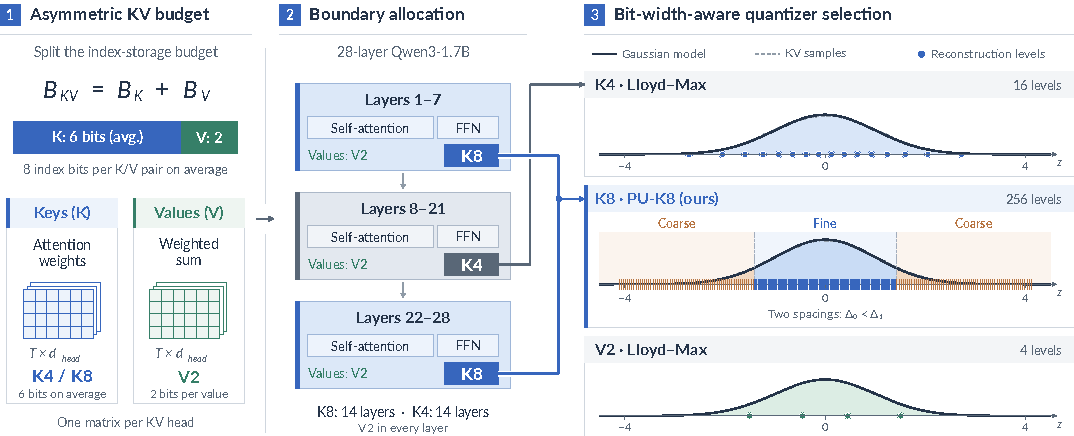
\includegraphics[width=\textwidth]{figures/kv_cache_overview.pdf}
\caption{Boundary 배치의 혼합 정밀도 KV 캐시에 통합한 하드웨어 인지형 K8 코덱. 연결선은 각 레이어 그룹의 K 정밀도를 고정된 코덱에 연결하며, K4/V2에는 Lloyd--Max를 유지한다.}
\label{fig:overview}
\end{figure*}

\section{배경 및 연구 동기}
\label{sec:background}
\subsection{키와 값의 양자화 오차}
스케일된 내적 어텐션은 다음과 같다~\cite{attention}.
\begin{equation}
 O=\operatorname{softmax}\!\left(\frac{QK^\top}{\sqrt{d}}\right)V,
 \label{eq:bg-attention}
\end{equation}
여기서 $Q$, $K$, $V$는 각각 쿼리, 키, 값이며, $d$는 키의 차원이다. 인과적 마스킹은 생략하였다. 키 양자화는 내적을 바꾸므로 지수함수를 정규화한 소프트맥스 가중치에도 영향을 준다. 반면 $Q$와 $K$가 고정되어 있을 때 값의 오차는 가중합에 선형적으로 반영된다. 이는 K/V 정밀도를 비대칭으로 설정하는 근거가 되지만, 키 오차가 항상 더 지배적이라는 뜻은 아니다.

\subsection{레이어별 양자화 민감도}
KV 양자화 민감도는 레이어마다 다르므로~\cite{kvtuner}, 고정된 캐시 예산에서 일부 레이어에 더 높은 정밀도를 배정할 수 있다. 본 연구에서는 K8과 K4를 혼합하여 평균 K6 정밀도를 유지하고, 모든 값에는 V2를 사용한다. Odd와 Boundary는 실험한 배치 방식이며 최적이라고 가정하지 않는다. 비교에는 동일한 레이어 마스크를 사용한다.

\subsection{코덱 실행 비용}
기존 K8 구현에서 Lloyd--Max 인코딩은 경계 비교와 복원 레벨 선택을 사용하고, LUT 디코딩은 선택된 레벨을 읽는다. 구간별로 균일한 레벨을 사용하면 산술 인덱싱과 네이티브 HVX 복원이 가능하다. 두 K8 코덱은 모두 좌표당 한 바이트를 저장하며, K4/V2는 기존 패킹 경로를 유지한다. 따라서 동일한 저장 정밀도에서도 양자화 레벨의 구조와 실행 경로에 따라 코덱 비용이 달라진다.

\section{하드웨어 인지형 K8 코덱 설계}
\label{sec:method}
\subsection{개요}
그림~\ref{fig:overview}의 세 패널은 저장 예산과 실제 코덱의 관계를 보여준다. 왼쪽 패널의 $B_K$와 $B_V$는 키와 값의 인덱스 저장 예산을 뜻하므로, $B_{KV}=B_K+B_V$에는 FP16 스케일이 포함되지 않는다. 캐시의 각 차원은 토큰 수 $T$, KV 헤드 수 $n_{\mathrm{heads}}$, 헤드 차원 $d_{\mathrm{head}}$이다. 레이어 절반에 K8을, 나머지에 K4를 배정하면 평균 키 정밀도는 6비트가 되며, 값에는 모두 V2를 사용한다.

가운데 패널은 28개 레이어 중 처음 7개와 마지막 7개에 K8을 배정하는 Boundary 배치를 보여준다. 그림에서는 레이어 번호를 1부터 $L$까지 표시하지만, 실험 마스크의 인덱스는 0부터 시작한다. 동일한 저장 예산에서 Odd 배치도 평가한다. 이 배치들은 양자화기 구현을 비교하기 위해 사용한 정밀도 할당 방식이다.

연결선은 각 레이어 그룹에 배정된 키 정밀도를 고정된 코덱에 연결한다. K4에는 Lloyd--Max를, K8에는 PU-K8을 사용하며, 모든 값에는 Lloyd--Max V2를 유지한다. 표준화된 축 $z=\sqrt{d}\,y$는 아래에서 사용하는 정규화·회전 좌표 $y$의 스케일을 조정한 것이다. 분포도에는 샘플 밀도와 설계용 가우시안 모델을 실제 FP16 복원 레벨과 함께 표시하였다. 다음 절에서는 산술 인덱싱과 네이티브 HVX 디코딩을 설명한다.

\subsection{양자화 레벨과 산술 인덱싱}
제안하는 키 캐시는 Lloyd--Max K4와 PU-K8을 사용한다. 비트 폭 $p$에 따른 양의 복원 레벨은 다음과 같다.
\begin{equation}
 \boxed{\ell_p^+(j)=\begin{cases}
  \mathcal{L}_4^+[j],&p=4,\\
  a_r+k\Delta_r,&p=8.
 \end{cases}}
 \label{eq:level}
\end{equation}
K4에서 $\mathcal{L}_4^+$는 $j\in\{0,\ldots,7\}$로 인덱싱되는 양의 Lloyd--Max 레벨 8개를 포함하며, 임계값 기반 인코더를 유지한다. K8에서는 $j=64r+k$이며, 구간 $r\in\{0,1\}$, 구간 내 인덱스 $k\in\{0,\ldots,63\}$, 오프셋 $a_r$, 간격 $\Delta_r$를 사용한다. 음의 레벨은 부호를 반전하여 얻는다. K8 식은 반올림 전의 레벨 격자를 나타내며, 곱셈과 덧셈은 각각 FP16으로 반올림한다.

네 개의 계수는 가우시안 근사 $\mathcal{N}(0,1/d)$에서 스칼라 평균제곱오차(MSE)를 최소화하도록 오프라인에서 결정하며, KV 샘플이나 PPL 기반 튜닝은 사용하지 않는다.

\emph{산술 인덱싱.} 정규화·회전 좌표 $y$에 대해 $m=|y|$로 둔다. 경계 $\tau$는 $(r,k)=(0,63)$과 $(1,0)$에서 FP16으로 반올림한 두 레벨의 중간값이다. 구간은 다음과 같이 선택한다.
\begin{equation}
 \boxed{r=\begin{cases}
  0,&m\leq\tau,\\
  1,&m>\tau.
 \end{cases}}
 \label{eq:region}
\end{equation}
구간 내 인덱스는 다음과 같다.
\begin{equation}
 \boxed{k=\clip\!\left(\left\lfloor(m-a_r)\dfrac{1}{\Delta_r}+0.5\right\rfloor,0,63\right)}
 \label{eq:index}
\end{equation}
위의 내림 연산 규칙에서는 두 인덱스의 정확한 중간값을 큰 쪽 인덱스로 반올림한다. 실제 실행에서는 저장된 역수와 중간 단계의 FP16 반올림을 사용하므로, 인덱스 경계 부근에서 선택 결과가 달라질 수 있다.

% Keep the decoder paragraph together in the Korean review layout.
\Needspace{11\baselineskip}
\subsection{HVX 산술 디코더}
네이티브 HVX 디코더는 저장된 각 바이트에서 $r$과 $k$를 추출하고, FP16 곱셈과 덧셈을 분리하여 $a_r+k\Delta_r$를 복원한다. 이후 부호와 노름 보정에 사용되는 유효 FP16 스케일을 적용하여 기존 어텐션 경로에 전달할 FP16 타일을 생성한다. 벡터화된 디코딩은 레벨 테이블 로드와 좌표별 스칼라 반복문을 제거한다. 계수 데이터는 FP16 값 4개(8바이트)로, FP16 항목 256개로 구성된 코드북(512바이트)을 대체한다.

\section{실험 방법}
실험에는 Qwen3-1.7B~\cite{qwen3}(W4A16)를 사용하였으며, Galaxy S26 Ultra(SM8850)에서 실행하였다. QAIRT 2.48.0.260626과 버스트 모드의 HTP 백엔드를 사용하였다. 추론은 단일 시퀀스로 수행하며, 성능 및 PPL 평가의 컨텍스트 용량은 1024이다. Odd와 Boundary 배치에서 동일한 레이어 마스크를 적용하여 PU-K8과 Lloyd--Max K8을 비교하였다. 가중치, 활성값 인코딩, 회전, 노름 보정 및 K4/V2 경로는 고정하였다.

성능 평가에는 프롬프트 897토큰과 생성 128토큰을 사용하였다. 각 실행은 전체 워밍업, 캐시 초기화, 측정 세션으로 구성된다. TTFT에는 모델 로딩 시간이 포함되지 않으며, 디코딩 처리량은 프리필 이후 자기회귀 단계의 총 소요 시간으로 127을 나누어 계산한다. Lloyd--Max 비교에서는 실행 순서의 영향을 상쇄하도록 순서를 배치하여 구성별로 10회의 측정 세션을 수행하였으며, 실행 사이에는 10초의 대기 시간을 두었다. 평균을 보고하고, 개선율은 구성별 평균으로 계산하였다. 동일한 세션 로그에서 호스트가 관측한 QNN 그래프 호출 경과 시간과 나머지 실행 시간을 구분하였다.

재사용한 WikiText-2~\cite{wikitext} 기준 구간 4개(각 1024토큰)의 PPL을 교사 강제(teacher forcing) 방식으로 평가하였다. 바이너리는 성능 평가와 동일하며, 구간별 1회 평가로 구성당 4092개의 대상 토큰을 채점하였다. 전체 PPL은 네 구간의 토큰 평균 음의 로그우도(NLL)에 지수 함수를 적용한 값이다. Uniform K8 비교는 Odd 배치의 별도 문서 4개에서도 PPL을 평가하였다.

Needle-in-a-Haystack(NIAH) 검색 평가에는 6자리 정답 코드를 삽입한 고정 WikiText-2 배경 문서 10개를 사용하였다. 삽입 깊이는 0, 25, 50, 75, 100\%의 다섯 가지이며, 컨텍스트 용량은 1K, 2K, 4K, 8K토큰이다(1K = 1024). 각 구성은 200개의 프롬프트로 평가하며, 각 프롬프트에서 비사고(non-thinking) 모드의 그리디 생성으로 한 번씩 디코딩하였다. 최대 64개의 출력 토큰을 확보하기 위해 프롬프트 길이를 컨텍스트 용량에서 64토큰을 뺀 범위 이내로 제한하였다. 정답으로 인정하려면 출력에서 독립된 6자리 코드가 정확히 하나 추출되어야 하며, 이 코드가 정답과 일치해야 한다. FP16 KV/어텐션, TurboQuant K4/V4, 그리고 Boundary 배치에서 K8/K4와 V2를 사용하는 두 구성을 비교하였다.

% Keep the results heading with its opening comparison.
\Needspace{5\baselineskip}
\section{결과 및 분석}
\subsection{종단 간 성능 및 품질}
PU-K8을 가우시안 모델에서 스칼라 복원의 MSE가 더 낮은 Lloyd--Max K8과 비교하였다. 이 비교는 전체 구현을 평가한다.

\begin{figure}[t]
\centering
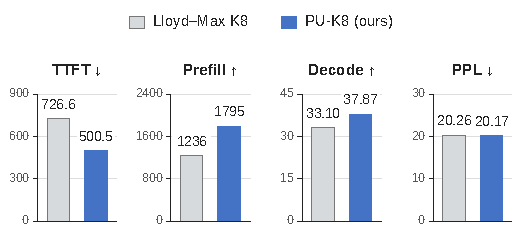
\includegraphics[width=\columnwidth]{figures/kv_cache_performance.pdf}
\caption{Boundary 배치의 성능과 기준 구간 PPL. TTFT(ms)와 처리량(tokens/s)은 프롬프트 897토큰과 생성 128토큰을 사용한 구성별 10회 측정의 평균이다. 백분율은 Lloyd--Max K8 대비 변화율이다.}
\label{fig:performance}
\end{figure}

그림~\ref{fig:performance}에서 Boundary 배치의 PU-K8은 평균 TTFT를 31.12\% 줄이고, 프리필 및 디코딩 처리량을 각각 45.22\%, 14.41\% 높였다. 별도의 Odd 배치 실험에서는 TTFT가 32.62\% 줄었으며, 프리필 및 디코딩 처리량은 각각 48.49\%, 13.61\% 높아졌다. 평가한 기기에서 두 레이어 마스크 모두 속도 향상이 관측되었다.

동일한 Boundary 세션에서 평균 누적 QNN 그래프 호출 시간은 프리필 중 697.47\,ms에서 475.11\,ms로, 생성 토큰당 28.43\,ms에서 24.63\,ms로 줄었다. 전체 토큰당 지연은 30.21\,ms에서 26.41\,ms로 줄었으며, 나머지 시간은 약 1.78\,ms로 유지되었다. 따라서 시간 감소는 실행과 스케줄링·대기 시간을 포함하는 그래프 호출 내부에 집중된다.

\begin{table}[!ht]
\caption{Odd에서 Boundary 배치로 변경했을 때의 기준 구간 PPL 감소.}
\label{tab:lm-ppl}
\centering
\setlength{\tabcolsep}{4pt}
\begin{tabular}{@{}lrrr@{}}
\toprule
K8 코덱 & \shortstack{Odd\\PPL $\downarrow$} & \shortstack{Boundary\\PPL $\downarrow$} & \shortstack{감소율\\(\%)}\\
\midrule
Lloyd--Max & 23.19 & \textbf{20.26} & 12.65\\
PU-K8 & 23.61 & \textbf{20.17} & 14.58\\
\bottomrule
\end{tabular}
\end{table}

재사용한 네 개의 기준 구간에서(표~\ref{tab:lm-ppl}), Boundary 배치는 Odd 대비 PPL을 Lloyd--Max에서 12.65\%, PU-K8에서 14.58\% 낮췄다. PU-K8의 PPL은 Lloyd--Max보다 Odd 배치에서 1.81\% 높고 Boundary 배치에서 0.45\% 낮아, 전체 PPL의 순위가 바뀐다. Odd에서는 Lloyd--Max가 세 구간에서 더 낮은 PPL을 보였으며, Boundary에서는 각 코덱이 두 구간에서 더 낮은 PPL을 보였다.

\subsection{Needle-in-a-Haystack 검색}
그림~\ref{fig:niah}는 구성별 200개 프롬프트의 정답 코드 추출 정확도를 보여준다. Boundary PU-K8은 93.5\%로, Boundary Lloyd--Max K8의 95.5\%보다 2.0\%p 낮다. TurboQuant K4/V4는 81.0\%이다.

\begin{figure*}[t]
\centering
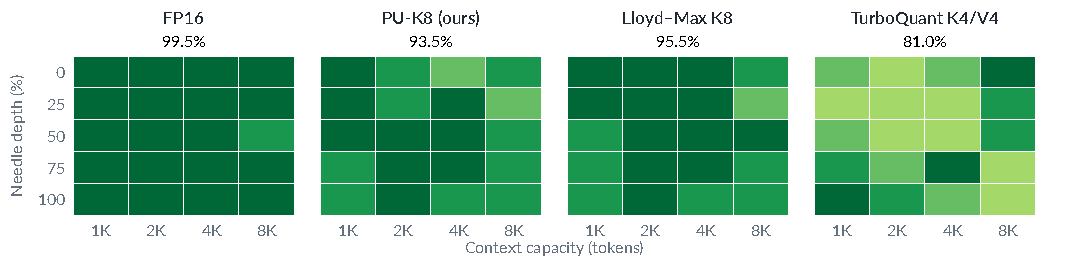
\includegraphics[width=\textwidth]{figures/kv_cache_niah_heatmap.pdf}
\caption{Qwen3-1.7B의 NIAH 정답 코드 추출 정확도(셀당 10개 사례). 두 K8 코덱은 Boundary 배치를 사용하며, 세 양자화 구성의 KV 캐시 저장 예산은 각 컨텍스트 용량에서 동일하다.}
\label{fig:niah}
\end{figure*}

\Needspace{5\baselineskip}
\subsection{균일 양자화와의 비교}
균일 양자화 기준선은 하나의 간격을 갖는 대칭적인 256레벨 격자를 사용한다. 간격은 동일한 가우시안 모델에서 결정하고 FP16으로 고정하였으며, KV 데이터나 PPL을 이용한 튜닝은 수행하지 않았다. 두 방식 모두 산술 HVX 디코더와 동일한 Odd 배치를 사용하므로, 동일한 배포 조건에서 단일 구간과 두 구간 양자화를 비교할 수 있다.

\begin{figure}[t]
\centering
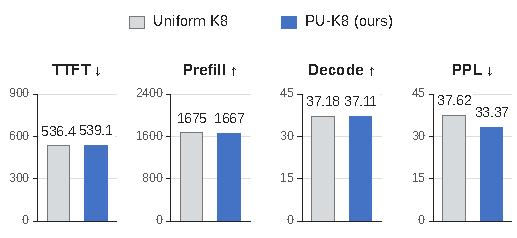
\includegraphics[width=\columnwidth]{figures/kv_cache_uniform_comparison.pdf}
\caption{Odd 배치에서 Uniform K8과의 비교. PPL은 별도의 문서 4개에서 평가하였다. 실행 성능은 구성별 3회 측정의 평균 $\pm$ 표본 표준편차이며, 프롬프트 897토큰과 생성 128토큰을 사용하였다. 백분율은 Uniform K8 대비 변화율이다.}
\label{fig:uniform}
\end{figure}

그림~\ref{fig:uniform}에서 PU-K8은 별도 문서 4개에서 PPL을 11.28\% 낮췄다. 같은 Odd 배치의 기준 구간에서는 Uniform 대비 PPL이 0.76\% 낮았다(23.79에서 23.61). 개선 폭은 평가 데이터에 따라 달라지며, 데이터 집합 간 PPL 절댓값은 직접 비교할 수 없다. 별도 문서 중 세 문서의 NLL이 개선되었지만, 순개선량의 대부분은 한 문서에서 발생하였다. 3회 성능 측정의 차이는 작고 측정 범위가 겹치므로, 어느 쪽도 명확한 속도 우위를 보이지 않는다.

\subsection{인코더 및 디코더 분석}
자기회귀 디코딩에는 새 KV의 인코딩, 캐시된 KV의 디코딩 및 어텐션이 포함된다. PU-K8은 반복적인 경계 비교와 레벨 선택을 산술 인덱싱과 복원으로 대체하여, 인코더 그래프의 ONNX 노드를 837개에서 76개로 줄인다. 동일한 입력을 사용한 단일 측정에서 SDK 실행 시간은 AR128(프리필)에서 52.21\%, AR1(토큰 생성)에서 9.78\% 짧았다(그림~\ref{fig:codec-costs}). AR128에서 더 큰 인코더 시간 감소가 나타난 점은 프리필에서 더 큰 속도 향상을 보인 결과와 부합한다.

캐시된 KV의 디코딩에서는 산술 복원이 LUT 로드를 제거한다. 256토큰 측정에서 SDK 실행 시간 감소는 1.38\%에 그쳤다. 동일한 입력 코드와 스케일을 사용할 때, 각 디코더는 해당 방법의 FP16 참조 결과와 비트 단위로 정확히 일치한다.

이러한 개별 측정은 전체 모델과 텐서 크기 및 실행 조건이 다르므로, 측정값을 합산하여 전체 속도 향상을 설명할 수 없다. 세션 로그는 그래프 호출 내부의 시간 감소를 보여주지만, 인코더·KV 디코더·어텐션 각각의 기여를 분리하지는 않는다.

\begin{figure}[!t]
\centering
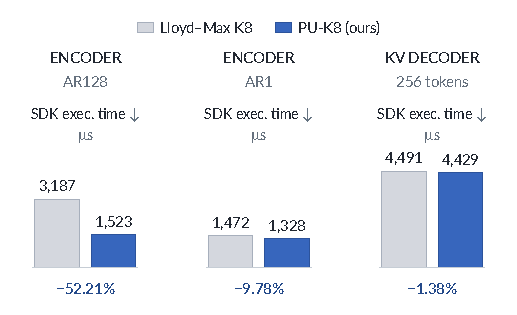
\includegraphics[width=\columnwidth,trim=0 6bp 0 6bp,clip]{figures/kv_cache_codec_costs.pdf}
\caption{AR128/AR1 인코더와 256토큰 KV 디코더의 단일 측정 SDK 실행 시간. 백분율은 Lloyd--Max K8 대비 변화율이며, 개별 측정 시간은 합산할 수 없다.}
\label{fig:codec-costs}
\end{figure}

% Keep the conclusion and references together in the final column.
\raggedend
\newpage
\section{결론}
KV 캐시의 효율은 저장 정밀도와 함께 코덱 실행 비용에 좌우된다. 평가한 모바일 NPU에서 PU-K8은 Lloyd--Max K8 대비 평균 TTFT를 31--33\% 줄이고 디코딩 처리량을 약 14\% 높였다. 관측된 품질 차이는 레이어 배치와 평가 데이터에 따라 달라진다. 추가 평가에는 더 큰 독립 데이터셋, 다양한 모델과 기기, 그리고 더 폭넓은 긴 컨텍스트 과제가 필요하다.

\begin{thebibliography}{00}
\bibitem{kivi} Z. Liu \emph{et al.}, ``KIVI: A tuning-free asymmetric 2bit quantization for KV cache,'' arXiv:2402.02750, 2024.
\bibitem{turboquant} A. Zandieh, M. Daliri, M. Hadian, and V. Mirrokni, ``TurboQuant: Online vector quantization with near-optimal distortion rate,'' arXiv:2504.19874, 2025.
\bibitem{pwlq} J. Fang, A. Shafiee, H. Abdel-Aziz, D. Thorsley, G. Georgiadis, and J. Hassoun, ``Post-training piecewise linear quantization for deep neural networks,'' arXiv:2002.00104, 2020.
\bibitem{ptq4vit} Z. Yuan, C. Xue, Y. Chen, Q. Wu, and G. Sun, ``PTQ4ViT: Post-training quantization for vision transformers with twin uniform quantization,'' in \emph{Proc. ECCV}, 2022.
\bibitem{attention} A. Vaswani \emph{et al.}, ``Attention is all you need,'' in \emph{Advances in Neural Information Processing Systems}, vol. 30, 2017.
\bibitem{kvtuner} X. Li \emph{et al.}, ``KVTuner: Sensitivity-aware layer-wise mixed-precision KV cache quantization for efficient and nearly lossless LLM inference,'' in \emph{Proc. ICML}, PMLR, vol. 267, pp. 36451--36485, 2025.
\bibitem{qwen3} A. Yang \emph{et al.}, ``Qwen3 technical report,'' arXiv:2505.09388, 2025.
\bibitem{wikitext} S. Merity, C. Xiong, J. Bradbury, and R. Socher, ``Pointer sentinel mixture models,'' arXiv:1609.07843, 2016.
\end{thebibliography}
\end{document}
